%\subsection{Neutrino Beam}
\begin{figure}
\caption{Scheme of LBNF/DUNE neutrino beam production system. Source of figure: \cite{ref_LBNFweb}}
\label{fig:LBNF_nuBeam}
\centering
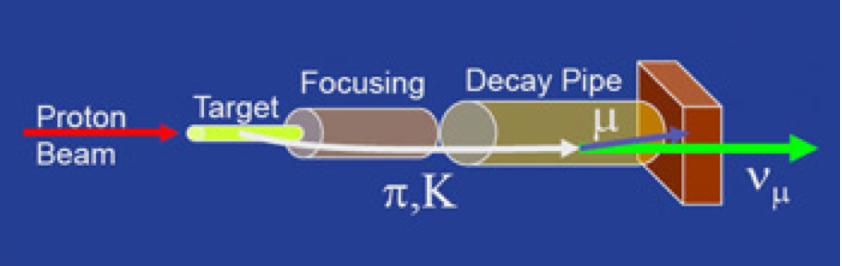
\includegraphics[width=0.45\textwidth, keepaspectratio=true]{figs/LBNF_nuBeam.png}  
\end{figure}
The LBNF neutrino beam will be the highest intensity neutrino beam ever created. The proton accelerator at Fermilab, which was already used in other experiments at Fermilab before, will produce the beam of protons. Then protons will hit a target and create pions and kaons through the strong interactions. Examples of dedicated reactions are: $p+p \rightarrow p+n+\pi^+$, $p+p \rightarrow p+\Delta^{++}+\pi^-$, $p+n \rightarrow p+p+\pi^-$, $p+n \rightarrow n+n+\pi^+$, $p+n \rightarrow p+\Delta^{-}+\pi^+$. \\ \\
%%%%%%%%%%%%%%%%%%%%%%%%%%%%%%%%%%%%%%%%%%%%%%%%%%%%%%
%% Feynman diagrams and descriptions of 
%% how the neutrinos were produced in the target 
%% are probably not necessary 
%%%%%%%%%%%%%%%%%%%%%%%%%%%%%%%%%%%%%%%%%%%%%%%%%%%%%%
%\begin{figure}
%\caption{Examples of the Feynmann diagrams of charged pion and kaon productions in proton-proton scattering.}
%\label{fig:pionAndKaonProductions}
%\centering
%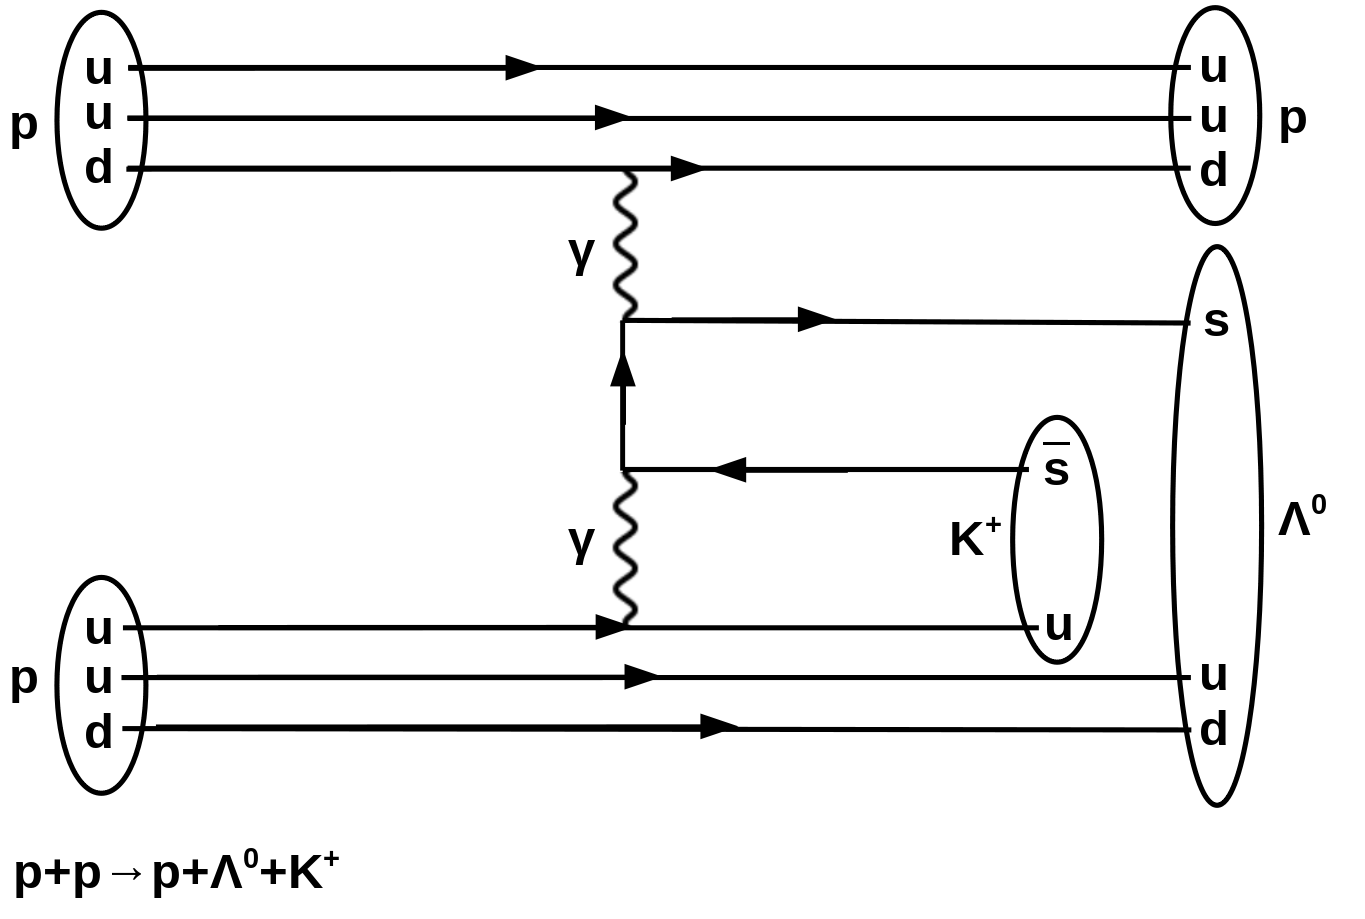
\includegraphics[width=0.48\textwidth, keepaspectratio=true]{figs/ppKaonProduction.png}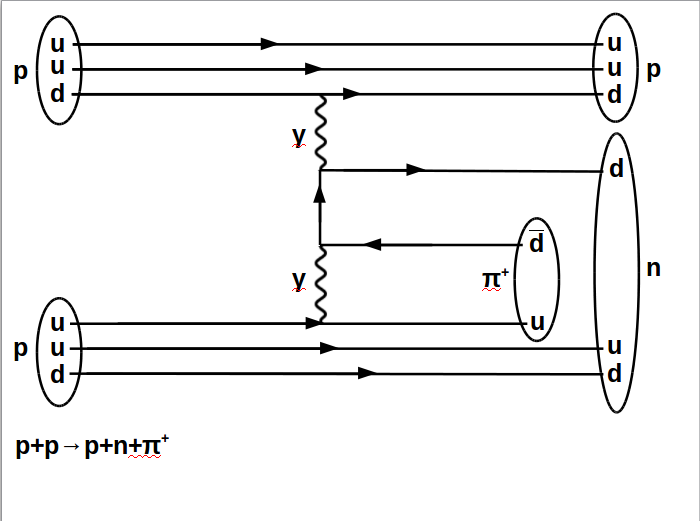
\includegraphics[width=0.48\textwidth, keepaspectratio=true]{figs/ppPionProduction.png}  
%\end{figure}
%In more general words, one quark from the accelerator beam proton scatters on the other quark from the proton or neutron of the target substance as shown at fig. \ref{fig:pionAndKaonProductions}. They exchange gluon which produces quark-antiquark pair. At this moment, the system has seven quarks and one antiquark. The antiquark pairs up with one of the quarks participating in the reaction and the remaining six quarks make two baryons in a way to satisfy color charge neutrality in final particles.  The charged pions have quark compositions $\pi^+ = u\bar{d}$ and $\pi^- = \bar{u}d$ and can be produced with the reactions which only include first generation quarks. The formulas of charged kaons are $K^+ = u\bar{s}$, $K^- = \bar{u}s$. Thus, to produce kaons, the gluon has to produce $s\bar{s}$ pair. 
%\begin{figure}
%\caption{Feynmann diagrams of charged pion and kaon decays to muon and muon antineutrino weakly through W-boson}
%\label{fig:pionAndKaonDecays}
%\centering
%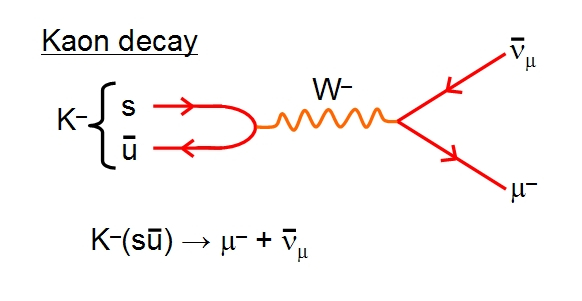
\includegraphics[width=0.45\textwidth, keepaspectratio=true]{figs/kaonDecay.jpg}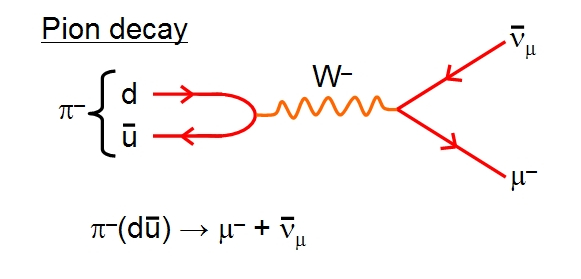
\includegraphics[width=0.45%\textwidth, keepaspectratio=true]{figs/pionDecay.jpg} 
%\end{figure}
After the mesons are created, they go through the focusing system and decay into the decay pipe as $\pi^+ \rightarrow \mu^+\nu_\mu$, $\pi^- \rightarrow \mu^-\bar{\nu_\mu}$, $K^+ \rightarrow \mu^+\nu_\mu$, $K^- \rightarrow \mu^-\bar{\nu_\mu}$. The branching ratios of charged pions and kaons to decay into $\mu^+\nu_\mu$($\mu^-\bar{\nu_\mu}$) are $(>99.9)\%$ and $(63.55\pm0.011)\%$ respectively \cite{ref_PDG}; therefore, most neutrinos produced into the decay pipe will be muon neutrinos. (While the neutral kaons can also be produced in the target and later decay to pions which could further decay and produce muon neutrinos, the focusing can be applied on charged particles only and therefore neutral particles produced would not contribute to the neutrino beam production unless they decay quickly to charged particles. Neutral pions, $\pi^0$s, are very likely to be produced as well but they decay as $\pi^0 \rightarrow \gamma\gamma$ and, therefore, can not contribute to the neutrino production.) It is important for the beam production system to operate in both neutrino and antineutrino modes by choice to probe Formula \ref{eq:P_bigFormula} for both cases, and the beam production system of the LBNF will be capable of this.\\ \\
After being produced in the reactions described above, the neutrinos will be detected in the ND at Fermilab. Then the neutrinos will travel 1300 km through the Earth's crust and will be detected at SURF in South Dakota.\\  \\
One of the most important beam requirements is high intensity to produce a large enough number of neutrinos to perform intended measurements. Beam power of 1.07 MW is expected in the beginning of the experiment with schedule upgrades to 2.4 MW which is four times larger than the highest beam intensity from other experiments of this kind (Tab. \ref{tab:compareExps}). Energies of produced neutrinos must cover the first and the second oscillation nodes which corresponds to energies of 0.5-10 GeV for a baseline of 1300 km (Fig. \ref{fig:LBNF_oscProbability}). Corresponding proton energies are 60-120 GeV.\\ \\
